\documentclass[letterpaper,12pt]{article}
\usepackage{array}
\usepackage{threeparttable}
\usepackage{geometry}
\usepackage{amsmath}
\geometry{letterpaper,tmargin=1in,bmargin=1in,lmargin=1.25in,rmargin=1.25in}
\usepackage{fancyhdr,lastpage}
\pagestyle{fancy}
\lhead{}
\chead{}
\rhead{}
\lfoot{}
\cfoot{}
\rfoot{\footnotesize\textsl{Page \thepage\ of \pageref{LastPage}}}
\renewcommand\headrulewidth{0pt}
\renewcommand\footrulewidth{0pt}
\usepackage[format=hang,font=normalsize,labelfont=bf]{caption}
\usepackage{listings}
\lstset{frame=single,
  language=Python,
  showstringspaces=false,
  columns=flexible,
  basicstyle={\small\ttfamily},
  numbers=none,
  breaklines=true,
  breakatwhitespace=true
  tabsize=3
}
\usepackage{amsmath}
\usepackage{amssymb}
\usepackage{amsthm}
\usepackage{harvard}
\usepackage{setspace}
\usepackage{float,color}
\usepackage[pdftex]{graphicx}
\usepackage{hyperref}
\hypersetup{colorlinks,linkcolor=red,urlcolor=blue}
\theoremstyle{definition}
\newtheorem{theorem}{Theorem}
\newtheorem{acknowledgement}[theorem]{Acknowledgement}
\newtheorem{algorithm}[theorem]{Algorithm}
\newtheorem{axiom}[theorem]{Axiom}
\newtheorem{case}[theorem]{Case}
\newtheorem{claim}[theorem]{Claim}
\newtheorem{conclusion}[theorem]{Conclusion}
\newtheorem{condition}[theorem]{Condition}
\newtheorem{conjecture}[theorem]{Conjecture}
\newtheorem{corollary}[theorem]{Corollary}
\newtheorem{criterion}[theorem]{Criterion}
\newtheorem{definition}[theorem]{Definition}
\newtheorem{derivation}{Derivation} % Number derivations on their own
\newtheorem{example}[theorem]{Example}
\newtheorem{exercise}[theorem]{Exercise}
\newtheorem{lemma}[theorem]{Lemma}
\newtheorem{notation}[theorem]{Notation}
\newtheorem{problem}[theorem]{Problem}
\newtheorem{proposition}{Proposition} % Number propositions on their own
\newtheorem{remark}[theorem]{Remark}
\newtheorem{solution}[theorem]{Solution}
\newtheorem{summary}[theorem]{Summary}
%\numberwithin{equation}{section}
\bibliographystyle{aer}
\newcommand\ve{\varepsilon}
\newcommand\boldline{\arrayrulewidth{1pt}\hline}
\setlength{\parindent}{4em}
\setlength{\parskip}{0.5em}
\renewcommand{\baselinestretch}{2.0}
\setlength{\abovedisplayskip}{1pt}
\setlength{\belowdisplayskip}{1pt}
\usepackage{indentfirst}

\begin{document}

\begin{flushleft}
  \textbf{\large{Methods and Initial Results}} \\
  MACS 30200\\
  Soo Wan Kim
\end{flushleft}
\section{Introduction}

In this paper I investigate the relationship between fatalities from covert air strikes on militant groups and subsequent timing of attacks by millitants, using Yemen as a case study. Specifically, I look at the effects of fatalities from all covert air strikes in Yemen from 2002 to the end of 2015 on the intervals in number of days between one terrorist incident in Yemen to another between March 2012 and the end of 2015. In addition, I only address attacks carried out by the militant group al-Qaeda in the Arabian Peninsula (AQAP), one of the main perpetrators of terrorist and insurgent violence in the Arabian Peninsula and also the primary target of counter-terror air strikes in Yemen.

Previously, I proposed using data from Afghanistan, Pakistan, Somalia, and Yemen, but given the varying and complex political, economic and social situations in each of the four countries I decided to focus on a single country instead. To further control for variables, I examine terrorist incidents occurring only after the Yemeni Revolution, which is connected to the broader Arab Spring phenomenon and took place roughly between January 27, 2011 and February 27, 2012. Due to lack of data and detailed knowledge, I could not control for the myriad complex developments occuring in Yemen since 2012, including major military offensives by AQAP and counter-offensives by the Yemeni and Saudi regimes. Thus, my models, which only account for covert strike fatalities, are unlikely to explain most of the variation in the timing of attacks. Also, due to the very high frequency of attacks in certain periods, the timing of attacks as measured in days may not be the most useful feature to study for the purpose of investigating the effectiveness of covert targeted killings in counter-terror and counter-insurgency operations. Either a more fine-grained measure in hours or even minutes, or a different measure of militant capabilities, such as lethality of attacks, could provide more useful insight.

\section{Data}

\subsection{AQAP attacks}

Data on AQAP attacks came from the Global Terrorism Database (GTD) managed at the University of Maryland. The GTD is one of the most detailed and comprehensive data sources for terrorist incidents around the world, and is freely accessible and extensively documented. The GTD defines terrorism as the ``\textit{the threatened or actual use of illegal force and violence by
a non‐state actor to attain a political, economic, religious, or social goal through fear, coercion,
or intimidation}." Its criteria for inclusion in the database include, roughly speaking, intentionality on the part of the perpetrator, use or threat of violence, and sub-national actors as perpetrators. This broad definition of terrorism covers essentially all violent offensives by AQAP. While the GTD allows filtering based on more narrow criteria for what constitutes terrorism, it was not necessary for this study as I am interested in AQAP's offensive capabilities as a whole, not just their use of terrorist tactics.

Within the GTD I looked only at observations for incidents that took place in Yemen between March 1, 2012 and the end of 2015 for which the first perpetuating group is coded as "Al-Qaida in the Arabian Peninsula" or "Al-Qaida in Yemen" (a precursor to AQAP). In addition, I only used observations where the attribution of the attack to the group is not based on speculation or dubious sources ($guncertain1$ = 0). Based on these specifications, the number of individual terrorist attacks was 537. Because the unit of analysis for the timing of attacks is one day, attacks occurring on the same date were treated as one attack. This reduced the number of observations to 362.

The table below shows the number of attacks occurring each year, and the average interval in days between each attack and the minimum and maximum intervals. To note, the number of attacks measure counts every attack separately, but the interval measures treat attacks occuring on the same day as a single incident. Thus, the minimum interval is 1 day rather than 0 days.\\

\begin {table}[H]
\begin{center}
\caption {Summary of attacks by AQAP in Yemen, 2012 - 2015}
\begin{tabular}{rlrrl}
  \hline
Year & \# Attacks & Avg. interval & Interval range \\ 
&&(days)&(days)\\
  \hline
2012 & 104 & 4.1 & 1, 38 \\ 
  2013 &  87 & 5.2 & 1, 31 \\ 
  2014 & 235 & 2.6 & 1, 20 \\ 
  2015 & 111 & 4.7 & 1, 41 \\ 
  \hline
  All & 537 & 3.9 & 1, 41 \\ 
   \hline
\end{tabular}
\end{center}
\end {table}

The following charts show the distribution of intervals between attacks ocurring between 2009 to 2015 and 2012 to 2015, respectively. There is a notable decrease in the overall spacing between attacks starting in 2012, which may have been caused by political changes or even by the stepping up of counter-terror operations in the region. From 2012 on there is significantly less variation, though the overall pattern appears to vary from year to year. In particular, attacks are more numerous in 2014 and occur in quicker succession than in any other year, as the summary table corroborates.

\begin{figure}[htb!]
  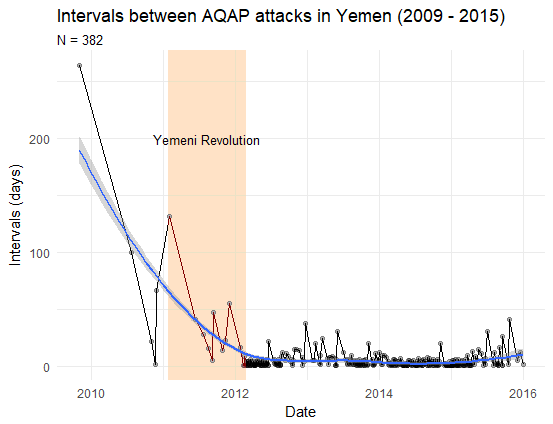
\includegraphics[width=3.5in]{intervals2009.png}
\end{figure}
\begin{figure}[htb!]
  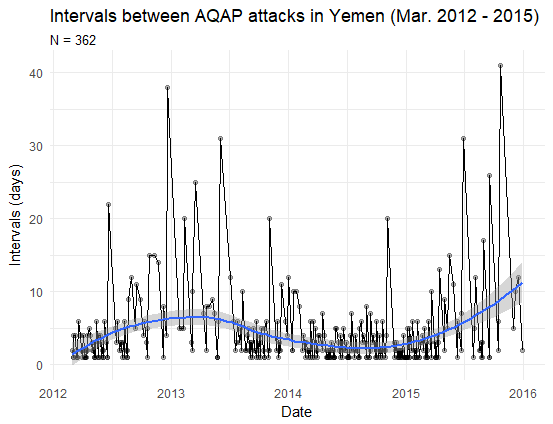
\includegraphics[width=3.5in]{intervals2012.png}
\end{figure}

The map below shows the geographical spread of attacks, and the bar plots show the breakdown of attacks in terms of target type, weapon type, and suicidal intent per year. Attack targets coded as "military" include members of Yemeni or foreign state armed forces, police, and terrorists or non-state militia. Government targets include government workers and politicians, whether part of the ruling regime or a rival political party. All other target categories were coded as "Other". In terms of weapon type, the "Unknown/Other" category includes various weapon types such as biological, chemical, or radiological weapons, fake weapons, sabotage equipment, motor vehicles excluding car bombs, and unknown. An attack was coded as "Yes" for a suicide attack if there was evidence that the attacker did not intend to survive the attack. This does not necessarily imply a suicide bombing or any other deliberate self-martyrdom mission where the goal is to strictly die while killing the target.

Most attacks occur in the east and south. The composition of targets is similar across years, though there is an appreciable 17\% drop in the percentage of attacks aimed at military targets between 2014 and 2015, accompanied by a corresponding increase in government targets. Most attacks were carried out using explosives and firearms. The percentage of attacks using explosives appears to have decreased slightly over the years, as does the percentage of suicide attacks.

\begin{figure}[htb!]
  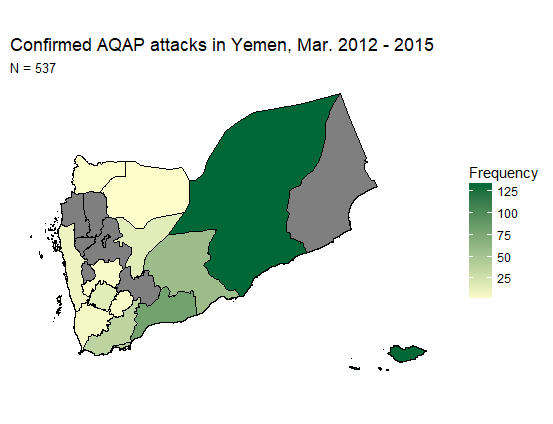
\includegraphics[width=3.5in]{attack_map.png}
\end{figure}

\begin{figure}[htb!]
  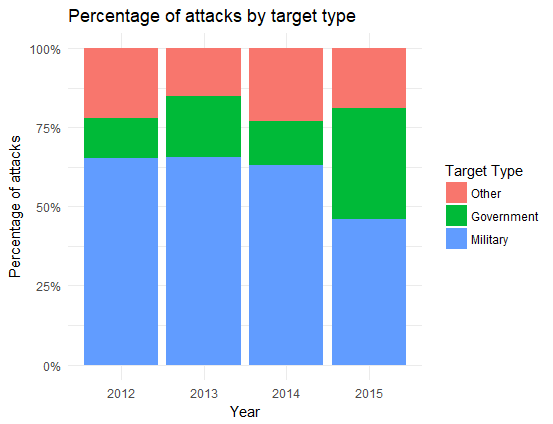
\includegraphics[width=3.5in]{attack_target.png}
\end{figure}

\begin{figure}[htb!]
  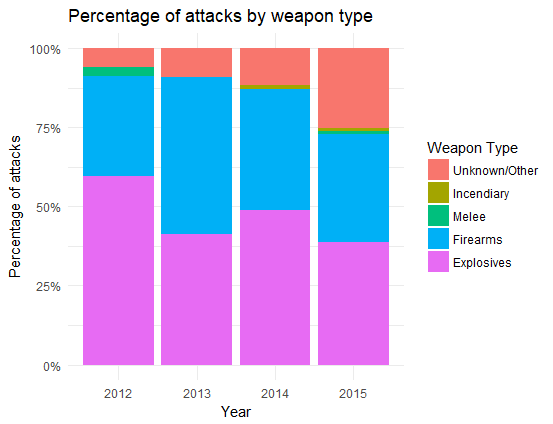
\includegraphics[width=3.5in]{attack_weapon.png}
\end{figure}

\begin{figure}[htb!]
  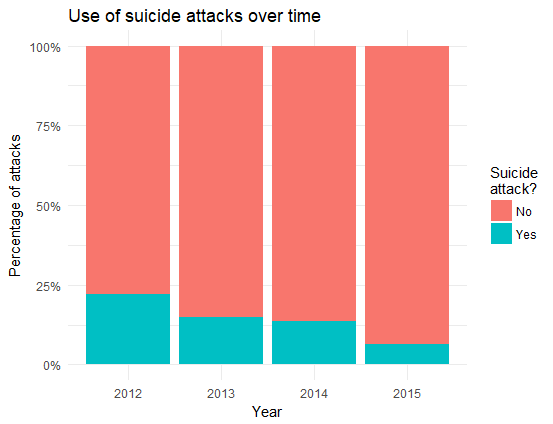
\includegraphics[width=3.5in]{attack_suicide.png}
\end{figure}

\subsection{Covert strikes}

Covert strikes data came from the Bureau of Investigative Journalism (TBIJ), which compiles reports of covert operations and related fatalities into an online database. TBIJ recorded 210 covert strike incidents between 2002 and 2015. An incident is any event where a covert operation was carried out in a single date and location. One incident can include multiple strikes. The operations include ground operations as well as drone and air strikes, but the majority of observations pertain to drone and air strikes. 

In addition, I obtained the list of group leaders killed per incident from the New America Foundation's online Drone Wars database. I joined the number of group leaders killed per incident to each observation in the TBIJ data by date. Although the NAF and TBIJ offer similar data, I use the TBIJ data as the main source as it includes more incidents within the timeframe of interest.

The following table shows the number of incidents per year, as well as the percentage of incidents confirmed to be US operations (as opposed to covert operations carried out by regional powers, such as Yemen or Saudi Arabia), averages for minimum and maximum fatality estimates, and the number of group leaders killed. Group leaders include senior leaders and prominent ideologues, and any other high-profile member of AQAP. 

\begin{table}[ht!]
\centering
\caption {Summary of covert strike incidents in Yemen, 2002 - 2015}
\begin{tabular}{rlrrrrr}
  \hline
Year & \# Incidents & \% US Confirmed & Avg. killed & Avg. killed & \# Leaders killed \\ 
& & & (min.) & (max.) &\\
  \hline
2002 &   1 & 100 & 6 & 6 & 2 \\ 
2009 &   3 & 100 & 28.3 & 30.7 & 2 \\ 
2010 &   7 & 28.6 & 2.1 & 5.3 & 1 \\ 
2011 &  25 & 40 & 6.8 & 9.4 & 8\\ 
2012 &  78 & 43.6 & 6 & 8.5 & 23 \\ 
2013 &  32 & 68.8 & 3.6 & 5.5 & 10 \\ 
2014 &  32 & 56.2 & 4.6 & 6.7 & 0 \\ 
2015 &  32 & 65.6 & 3.4 & 4.9 & 3 \\ 
  \hline
All & 210 & 52.9 & 5.3 & 7.5 & 49 \\ 
   \hline
\end{tabular}
\end{table}

The following chart shows the distribution of fatalities from covert strikes. The measure used is the average of the minimum and maximum estimates for each incident. We see that the number of deaths is typically below 20, and further, that the number of civilian deaths is very small compared to the number of militant deaths. This reflects the high precision of the weaponry and tactics, and possibly limitations in reporting.

\begin{figure}[htb!]
  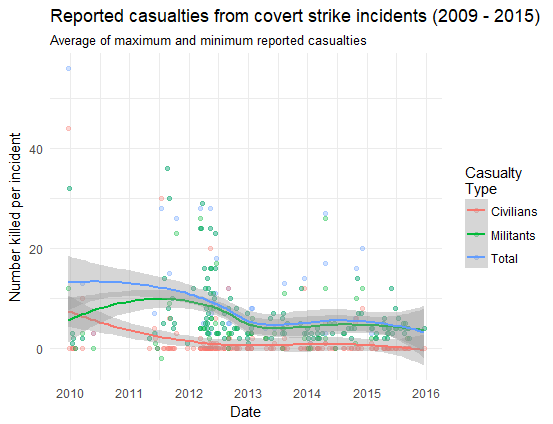
\includegraphics[width=3.5in]{strike_killed.png}
\end{figure}

The map of strike incident locations shows that the operations are carried out primarily in the east and south, which is consistent with the geographical spread of terrorist attacks.

\begin{figure}[htb!]
  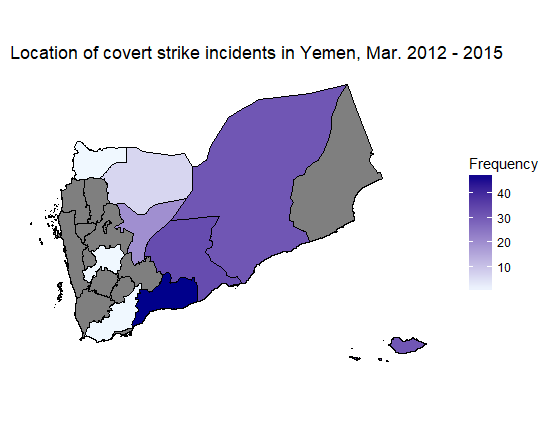
\includegraphics[width=3.5in]{strike_map.png}
\end{figure}

\section{Methods}
I test the following hypotheses:
\begin{itemize}
  \item $H_0$: Fatalities from covert air strikes have no effect on the intervals between attacks.
  \item $H_1$: An increase in fatalities from covert air strikes shortens the intervals between attacks.
  \item $H_2$: An increase in fatalities from covert air strikes lengthens the intervals between attacks.
\end{itemize}
I model the interval between one attack to another (in number of days) as a function of the cumulative effect of all covert strike fatalities incurred up to that point, using a simple linear model and a fixed effects model. For both models I make the following simplifying assumptions:
\begin{itemize}
  \item \textbf{Assumption 1}: The effects of any given strike only lasts for a certain number of days; after this period has passed, the group recovers from any deaths caused by that strike.
  \item \textbf{Assumption 2}: Within the period where a strike is still relevant, its effects depreciate each passing month.
  \item \textbf{Assumption 3}: The death of a group leader has a greater effect than the death of a non-leader.
  \item \textbf{Assumption 4}: When multiple group leaders are killed in the same strike, the effect is multiplicative rather than additive.
  \item \textbf{Assumption 5}: The effect of the death of a non-leader is similar for militants and civilians.
\end{itemize}
Despite obvious differences in public perception regarding civilian deaths versus militant deaths, I argue that assumption 5 is not unreasonable in this context as the number of civilian deaths from covert air strikes in Yemen is very small, as previously shown in the Data section. In addition, the line between civilians and militants are often blurred, especially when militants and surrounding communities work together.

Also, while geographical factors likely play a role, I do not address them in this analysis. Lastly, I assume attacks always occur in ordered sequence; that is, the interval between attacks is always greater than 0. I treat attacks occuring on the same day as a single attack. 

For the simple linear regression I estimate the following:
\[log\left(interval_t\right) = \beta_0 + \beta_1log\left(killed_{ct}\right) \]
where for each time period $t$ in which an attack has occurred, $interval_{t}$ is the period of time in days until the next attack, and $killed_{ct}$ is the cumulative effect of all covert strike fatalities incurred up to and including period $t$.

This culumative effect is modeled as:
$$killed_{ct} = \sum_{n=t-x}^{t} (1 + \alpha)^{K_n}killed_{n}(1-\delta)^{D_{n}}$$
where $x$ is some fixed cutoff in difference in days, $\alpha$ is the added effect of the death of a group leader, $K_{n}$ is the number of group leaders killed in period $n$, $killed_{n}$ is the number of covert strike fatalities in period $n$, and $\delta$ is a depreciation constant by which the effect of an attack in a period depreciates in each subsequent period (due to new recruits, replacements, forgetting, etc.). $D_{n}$ is the 30-day difference between periods $n$ and $t$; I assume that the effects of an attack depreciate on a monthly basis. $D$ is calculated as follows:
$$D_{n} = floor((t - n)/30)$$
Thus, if $x$ = 30 the cumulative effect covers the deaths caused by covert strikes in the last thirty days and there is no depreciation effect. For $D_{n} > 1$ there is a depreciation effect and more recent deaths are weighed more heavily.

The parameters were set arbitrarily as follows: 
$$\alpha = 0.1; \delta = 0.6$$
and time difference $x$ was set at 60 (2 months), 180 (6 months), and 360 (1 year), respectively.

The fixed effects model employs the same model and specifications, but with added year fixed effects.

\section{Results}
\noindent\textit{Simple linear regression model}

The signs and significance of the estimates were similar across specifications $x$ = 60, 180, and 360. I display the results for the model using $x$ = 180 below:

\begin{table}[!htb]
\centering
\begin{tabular}{rlrrrr}
  \hline
term & estimate & std.error & statistic & p.value \\ 
  \hline
(Intercept) & 1.54 & 0.13 & 11.64 & 0.00 \\ 
log(killed) & -0.07 & 0.04 & -1.74 & 0.08 \\ 
   \hline
\end{tabular}
\end{table}

The coefficient estimate indicates a very small negative association between the cumulative effect measure and the interval between attacks. A 1\% increase in the cumulative effect measure is associated with a 0.07\% decrease in the number of days until the next attack. In other words, a 100\% increase in the cumulative effect measure is expected to decrease the interval by only 7\%. In fact, the range in predicted intervals across cumulative effects is quite narrow, as the below plot shows. The association is significant at the 0.1 level. The R-squared value is low, at only 0.008876. \\

\begin{figure}[ht!]
  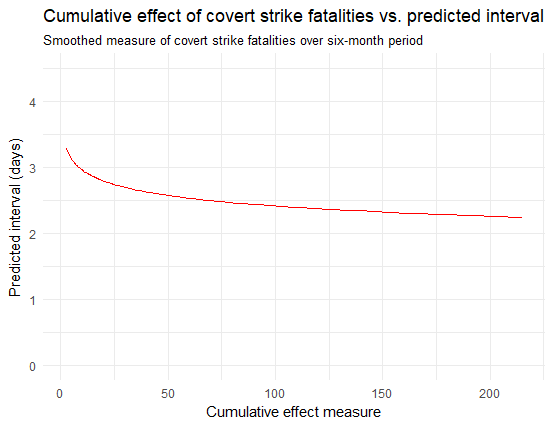
\includegraphics[width=3.5in]{pred_plot.png}
\end{figure}

\noindent\textit{Fixed effects model}

I estimate the same model as above with fixed year effects, using year 2012 as the baseline. Again, the signs and significance of coefficient estimates persisted across specifications  $x$ = 60, 180, and 360. The table below shows the output for the model setting $x$ = 180.

\begin{table}[htb!]
\centering
\begin{tabular}{rrrrr}
  \hline
Estimate & Std. Error & t value & Pr($>$$|$t$|$) \\ 
  \hline
(Intercept) & 1.9097 & 0.2328 & 8.20 & 0.0000 \\ 
  log(killed) & -0.1274 & 0.0508 & -2.51 & 0.0126 \\ 
  factor(year)2013 & -0.0087 & 0.1285 & -0.07 & 0.9461 \\ 
  factor(year)2014 & -0.3569 & 0.1112 & -3.21 & 0.0015 \\ 
  factor(year)2015 & -0.1940 & 0.1248 & -1.55 & 0.1210 \\ 
   \hline
\end{tabular}
\end{table}

Again, there is a small negative association between the cumulative effect measure and the attack interval. A 100\% increase in the cumulative effect measure is associated with a 12.7\% decrease in the number of days between attacks. The association is significant at the 0.05 level. In addition, relative to the base year 2012, years 2013 to 2015 are associated with slightly shorter intervals between attacks. The association is significant at the 0.01 level for year 2014. The R-squared is again low at 0.063.

\begin{figure}[htb!]
  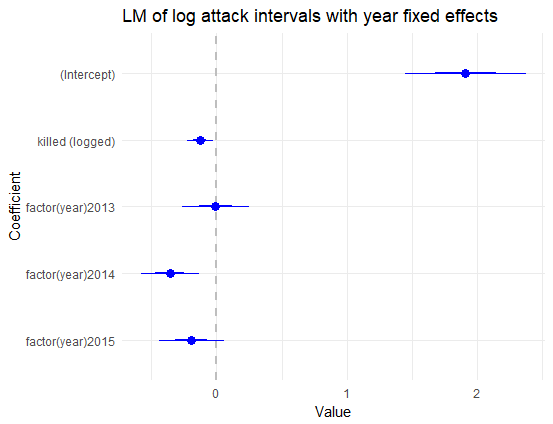
\includegraphics[width=3.5in]{coef_plot.png}
\end{figure}

\section{Discussion}

The results indicate a small but significant negative association between my cumulative effects measure and the interval between attacks occuring on different days. In other words, higher covert strike fatalities and greater rates of leadership decapitation slightly decreases the amount of time between attacks. This is consistent with the backlash theory that predicts that militant groups will react with greater aggression in response to targeted killings. However, more attacks in shorter periods could also indicate greater vulnerability. For instance, weakened militant groups could opt for easier, less carefully planned attacks that require less time to prepare but have less impact. The trends in the attacks support this theory to a limited extent; AQAP appears to be using explosives and suicide tactics less over time. Use of explosives and suicide attacks arguably requires more specific knowledge, greater training, and recruitment capabilities compared to other types of attacks, such as shootings or sabotage. On the other hand, the apparent change in tactics could also arise from other reasons not excluding random chance.

Regression results did not significantly differ when the period of relevance was changed from two months to six or twelve months. This is not surprising given that the depreciation rate was set at 60\%. More recent fatalities were weighed much more heavily than fatalities from older strikes. 

Lastly, attack intervals appear to differ from one year to another. This in addition to the small R-squared values indicate that the models used fail to account for important factors. A more refined model will take into account the volatile political situation in Yemen and other complex variations such as changes in military strategy and resource availability.

\end{document}